\documentclass[11pt]{article}

\usepackage{amsmath, amssymb, amsthm, graphicx}
\usepackage{fullpage}
\usepackage{natbib}
\usepackage{tikz}
\usetikzlibrary{arrows.meta, positioning}

\title{A Gentle Intro to Branch-and-Price:\\
From Linear Programming to Dantzig--Wolfe and Column Generation}
\author{Bayzhan Mukatay}
\date{}

\begin{document}

\maketitle

\begin{abstract}
Linear programs (LPs) can be solved efficiently at large scale and are a core tool
in optimization.
Mixed-integer linear programs (MILPs) extend LPs with integrality constraints and
capture a wide range of decision problems, but are much harder to solve.
Classical branch-and-bound is an exact method for MILPs, yet its efficiency
depends critically on the quality of the relaxation solved at each node.
This article introduces the idea of using stronger relaxations, obtained via
Dantzig--Wolfe decomposition and solved by column generation, to accelerate
branch-and-bound.
We begin with a high-level LP and MILP perspective, motivate the need for
decomposition using a driver--contract assignment model, and then describe how
branch-and-price leverages tighter relaxations.
Column generation is illustrated through the cutting-stock problem, following
the spirit of Chapters~2.2 and~8 of \emph{Integer Programming} by
Conforti, Cornu\'ejols, and Zambelli.
\end{abstract}

\section{Linear Programming as a Starting Point}

Linear programming (LP) considers problems of the form
\begin{align*}
    \max \quad & c^\top x \\
    \text{s.t.} \quad & Ax \le b, \\
    & x \ge 0,
\end{align*}
where $A \in \mathbb{R}^{m \times n}$, $b \in \mathbb{R}^m$, and
$x \in \mathbb{R}^n$.
LPs have a rich geometric and algorithmic theory:
\begin{itemize}
    \item the feasible region is a convex polyhedron;
    \item strong duality holds under mild conditions;
    \item there exist polynomial-time algorithms (e.g., interior-point methods);
    \item mature solvers can reliably handle very large LPs.
\end{itemize}
In practice, LPs are often the first modeling tool one reaches for: they are
expressive enough for many problems and can be solved at scale.

However, many real-world decisions are inherently discrete:
assigning drivers to routes, choosing which facility to open,
or deciding which pattern to use in cutting stock.
This leads naturally to mixed-integer linear programs.

\section{From LPs to MILPs: Why Integrality is Hard}

A mixed-integer linear program (MILP) adds integrality constraints to some
variables:
\begin{align*}
    \max \quad & c^\top x \\
    \text{s.t.} \quad & Ax \le b, \\
    & x_j \in \mathbb{Z} \text{ or } \{0,1\} \text{ for certain } j, \\
    & x_k \ge 0 \text{ (continuous) for others } k.
\end{align*}
The presence of integrality makes the feasible region \emph{nonconvex}: it is
a finite or countable set of points, or a union of such sets, rather than a
single polyhedron.
This has several consequences:
\begin{itemize}
    \item we cannot simply rely on convex optimization theory to solve MILPs;
    \item duality and strong convexity-based guarantees apply only to the LP relaxations;
    \item MILPs are NP-hard in general, and no polynomial-time algorithm is known.
\end{itemize}
We can still define an LP relaxation by dropping integrality constraints.
Its dual is well defined and useful, but it only characterizes the relaxed
problem, not the original MILP.

To see concretely why structure and decomposition matter, consider the following
motivating example.

\section{Motivating Example: Driver--Contract Assignment with Paths}

Suppose we have a set of drivers
\[
    D = \{d_1, d_2, \dots, d_n\},
\]
and a set of contracts
\[
    C = \{c_1, c_2, \dots, c_m\}.
\]
For each driver $d \in D$, we precompute a set of feasible paths (or schedules)
\[
    P_d = \{ p_{d,1}, p_{d,2}, \dots \}.
\]
Each path $p_{d,j} \in P_d$ is characterized by:
\begin{itemize}
    \item a subset of contracts covered: $C(p_{d,j}) \subseteq C$;
    \item a profit (or cost) $r_{d,j} \in \mathbb{R}$.
\end{itemize}

We want to choose exactly one path for each driver, and ensure that each contract
is covered at most once.
We also want to prioritize contract coverage, so we use a big-$M$-type objective
that heavily rewards paths covering more contracts.

Let $x_{d,j}$ be a decision variable indicating whether driver $d$ uses path
$p_{d,j}$.
In a pure integer model, we enforce $x_{d,j} \in \{0,1\}$; in the LP relaxation,
we allow $x_{d,j} \in [0,1]$.

We define a large constant
\[
    M = n \cdot \max_{d,j} |r_{d,j}| + 1,
\]
so that the contribution $M \cdot |C(p_{d,j})|$ dominates $r_{d,j}$ in the
objective.
The model is:
\begin{align*}
    \max \quad &
    \sum_{d \in D} \sum_{j \in P_d}
    \bigl( r_{d,j} + M \cdot |C(p_{d,j})| \bigr) x_{d,j} \\
    \text{s.t.} \quad
    & \sum_{j \in P_d} x_{d,j} = 1, \quad && \forall d \in D \quad
      \text{(each driver chooses exactly one path)} \\
    & \sum_{d \in D} \sum_{j \in P_d : c \in C(p_{d,j})} x_{d,j} \le 1,
      && \forall c \in C \quad
      \text{(each contract is covered at most once)} \\
    & x_{d,j} \in \{0,1\} \quad && \forall d \in D,\, j \in P_d.
\end{align*}

This is essentially a set-packing/assignment-type MILP.
The catch lies in the index sets $P_d$:
\begin{itemize}
    \item each driver $d$ may have a huge number of feasible paths $p_{d,j}$;
    \item $P_d$ is often generated implicitly (e.g., all feasible sequences of
          tasks or time windows), and is too large to enumerate in advance.
\end{itemize}
Even if we relax $x_{d,j}$ to be continuous in $[0,1]$ and consider the LP
relaxation, the resulting model may have an astronomical number of variables.
This illustrates two intertwined difficulties:
\begin{enumerate}
    \item the \emph{integrality} requirement makes the problem a MILP;
    \item the \emph{number of columns} (paths) is exponential, making naive LP
          or MILP formulations impractical.
\end{enumerate}

These issues motivate the use of decomposition techniques and algorithms
designed to work with implicitly defined variables.

\section{Branch-and-Bound: High-Level View}

Branch-and-bound (B\&B) is the standard exact method for MILPs.
At a high level:
\begin{enumerate}
    \item Start from the original MILP and relax integrality to obtain an LP.
    \item Solve this LP relaxation:
    \begin{itemize}
        \item if the LP is infeasible, the MILP is infeasible;
        \item if the LP solution is integral, it is optimal for the MILP;
        \item otherwise, the LP solution is fractional.
    \end{itemize}
    \item If the LP solution is fractional, choose a branching decision
          (e.g., $x_{d,j} \in \{0,1\}$ becomes two subproblems with
          $x_{d,j} =0$ and $x_{d,j}=1$).
    \item Recursively repeat on each subproblem:
    \begin{itemize}
        \item solve its LP relaxation;
        \item prune the node if the LP bound is worse than the best known integer solution;
        \item otherwise, branch again if the solution is still fractional.
    \end{itemize}
\end{enumerate}
The power of B\&B comes from \emph{pruning}:
if the relaxation at a node proves that no integer solution in that region can
beat the incumbent, the entire subtree can be discarded.

However, the efficiency of B\&B depends critically on the strength of the
relaxation:
\begin{itemize}
    \item if the LP relaxation is weak (feasible region much larger than the
          convex hull of $P_{IP}$), bounds are poor and pruning is rare;
    \item if the relaxation is tight, bounds are strong and many nodes can be
          eliminated early.
\end{itemize}
This observation motivates stronger relaxations and more sophisticated
formulations.

\section{Stronger Relaxations and a Geometric Illustration}

Let $P_{IP}$ be the integer-feasible region,
and let $P_{LP}$ be the standard LP relaxation region.
In many structured problems, we can exploit block structure to build an
intermediate region $P_{DW}$ such that
\[
    P_{IP} \;\subseteq\; P_{DW} \;\subseteq\; P_{LP}.
\]
Here $P_{DW}$ is the feasible region of a \emph{Dantzig--Wolfe} (DW) relaxation:
a convexification that captures the structure of blocks more faithfully than
the naive LP relaxation.

Figure~\ref{fig:geometry} provides a simple geometric illustration in two
dimensions.
A finite set of integer points (representing $P_{IP}$) is plotted explicitly.
Their convex hull $\operatorname{conv}(P_{IP})$ is shown as a tight polygon.
A larger polygon represents a looser LP relaxation $P_{LP}$ that contains the
convex hull but also many fractional points.
\begin{figure}[t]
\centering
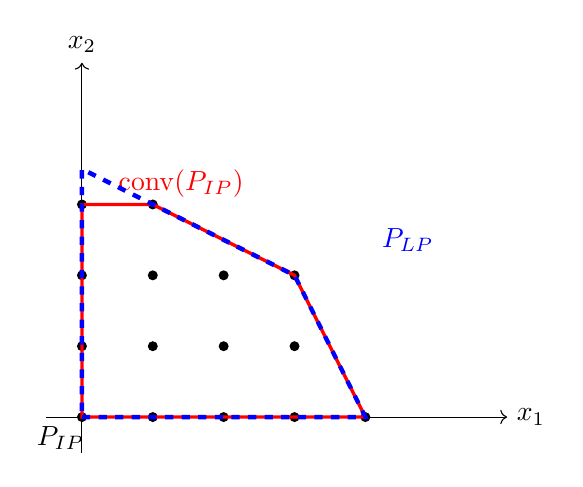
\begin{tikzpicture}[scale=0.9]

    % AXES
    \draw[->] (-0.5,0) -- (6,0) node[right] {$x_1$};
    \draw[->] (0,-0.5) -- (0,5) node[above] {$x_2$};

    % INTEGER FEASIBLE POINTS (black dots)
    \foreach \x/\y in {
        0/0,1/0,2/0,3/0,4/0,
        0/1,1/1,2/1,3/1,
        0/2,1/2,2/2,
        0/3,1/3,
        3/2
    }{
        \fill (\x,\y) circle (2pt);
    }
    \node at (-0.3,-0.3) {$P_{IP}$};

    % INTEGER HULL (red polygon) — drawn FIRST
    \draw[red, very thick]
        (0,0) --
        (4,0) --
        (3,2) --
        (1,3) --
        (0,3) -- cycle;
    \node[red] at (1.4,3.3) {$\mathrm{conv}(P_{IP})$};

    % LP RELAXATION POLYTOPE (blue dashed) — drawn SECOND (on top)
    \draw[blue, dashed, ultra thick]
        (0,0) --
        (4,0) --
        (3,2) --
        (0,3.5) -- cycle;
    \node[blue] at (4.6,2.5) {$P_{LP}$};

\end{tikzpicture}

\caption{
Integer-feasible region $P_{IP}$ (black points), its convex hull $\mathrm{conv}(P_{IP})$ (red polygon),
and the LP relaxation region $P_{LP}$ (blue dashed polygon) for the MILP defined by
$x_1 + 2x_2 \le 7$, $2x_1 + x_2 \le 8$, $x_1,x_2 \ge 0$.
The convex hull is strictly contained inside the LP relaxation, illustrating the relaxation gap.
}
\end{figure}




Branch-and-price is the method obtained by:
\begin{itemize}
    \item running branch-and-bound as usual;
    \item but at each node, solving a DW relaxation over a region like $P_{DW}$
          (rather than the standard LP relaxation over $P_{LP}$);
    \item using column generation to handle the large number of columns
          introduced by the DW reformulation.
\end{itemize}
Because $P_{DW}$ is a much tighter approximation of $P_{IP}$, the bounds at
each node are significantly stronger, leading to more pruning and a smaller
search tree.

\section{Dantzig--Wolfe and Column Generation via Cutting Stock}

The cutting-stock problem provides the classical and cleanest illustration
of Dantzig--Wolfe (DW) decomposition and column generation.
It is also the canonical model treated in Chapter~2.2 and Chapter~8 of
Conforti--Cornu\'ejols--Zambelli.

We begin by writing the \emph{full} mixed-integer model, then its LP
relaxation and dual, followed by the restricted master problem (RMP) and
the dual of the RMP (DRMP).
This will make clear why a dual-feasibility check certifies optimality of
the full LP, and how column generation emerges naturally.

\subsection{The Full Cutting-Stock MIP}

We are given:
\begin{itemize}
    \item roll width $W$,
    \item item types $i=1,\dots,m$ with width $w_i$ and demand $b_i$,
    \item cutting patterns $s \in \mathcal{S}$, where
          $s = (s_1,\dots,s_m) \in \mathbb{Z}_+^m$ satisfies
          $\sum_i w_i s_i \le W$.
\end{itemize}

Let $x_s \in \mathbb{Z}_+$ denote how many rolls are cut using pattern $s$.
The full MIP is
\begin{align}
\min \quad & \sum_{s\in\mathcal{S}} x_s
    \label{eq:full_mip_obj} \\
\text{s.t.}\quad
& \sum_{s\in\mathcal{S}} s_i x_s \;\ge\; b_i,
    && i=1,\dots,m, \label{eq:full_mip_demands} \\
& x_s \in \mathbb{Z}_+, && s\in\mathcal{S}. \label{eq:full_mip_int}
\end{align}

The difficulty is that $\mathcal{S}$ is enormous (exponential in $W$).

\subsection{Full LP Relaxation and Its Dual}

Relaxing integrality in \eqref{eq:full_mip_int} gives the full LP:
\begin{align}
\min \quad & \sum_{s\in\mathcal{S}} x_s \label{eq:full_lp_obj} \\
\text{s.t.}\quad
& \sum_{s\in\mathcal{S}} s_i x_s \;\ge\; b_i,
   && i=1,\dots,m, \label{eq:full_lp_demands} \\
& x_s \ge 0, && s\in\mathcal{S}. \label{eq:full_lp_nonneg}
\end{align}

Let $\pi_i \ge 0$ be the dual variables associated with
\eqref{eq:full_lp_demands}.
The full LP dual is:
\begin{align}
\max \quad & \sum_{i=1}^m b_i \pi_i
    \label{eq:dual_obj} \\
\text{s.t.}\quad
& \sum_{i=1}^m s_i \pi_i \;\le\; 1,
   && \forall\, s\in\mathcal{S}, \label{eq:dual_full_constraint} \\
& \pi_i \ge 0, && i=1,\dots,m.
    \label{eq:dual_nonneg}
\end{align}

The problem is now located in the \emph{dual constraints}:
there is one constraint \eqref{eq:dual_full_constraint} for
\emph{every pattern} $s\in\mathcal{S}$.
This dual is huge; solving the primal or dual directly is intractable.

\subsection{Restricted Master Problem (RMP)}

Column generation begins by selecting a small subset
$\mathcal{S}'\subset\mathcal{S}$.
We solve the RMP:
\begin{align}
\min \quad & \sum_{s\in\mathcal{S}'} x_s \label{eq:rmp_obj} \\
\text{s.t.}\quad
& \sum_{s\in\mathcal{S}'} s_i x_s \;\ge\; b_i,
    && i=1,\dots,m, \label{eq:rmp_demands} \\
& x_s \ge 0, && s\in\mathcal{S}'. \label{eq:rmp_nonneg}
\end{align}

Let $\pi_i$ be the dual variables of \eqref{eq:rmp_demands}.
The dual RMP (DRMP) is
\begin{align}
\max \quad & \sum_{i=1}^m b_i \pi_i
    \label{eq:drmp_obj} \\
\text{s.t.}\quad
& \sum_{i=1}^m s_i \pi_i \;\le\; 1,
    && \forall s\in\mathcal{S}', \label{eq:drmp_constraints} \\
& \pi_i \ge 0. \label{eq:drmp_nonneg}
\end{align}

The DRMP keeps \emph{only a subset} of the dual constraints of the full dual.

\subsection{Key Insight: A Dual Feasibility Test Certifies Optimality}

Let $(\pi_i)$ be the solution of the DRMP.
Two facts hold:

\begin{enumerate}
    \item \textbf{The DRMP is a relaxation of the full dual.}  
          It contains fewer constraints:  
          \[
             \{\text{DRMP constraints}\} \subseteq
             \{\text{full dual constraints}\}.
          \]
          Thus its feasible region is \emph{larger}, and its optimal objective
          value is \emph{at least as large} as the full dual optimum.

    \item \textbf{If the DRMP dual solution satisfies all full dual constraints
          \eqref{eq:dual_full_constraint}, then it is feasible for the full dual.}
\end{enumerate}

Combining the two:
\begin{quote}
If $(\pi_i)$ from the DRMP also satisfies every missing constraint
\eqref{eq:dual_full_constraint}, then it is optimal for the full dual and
certifies optimality of the full LP relaxation.
\end{quote}

This yields the \textbf{column generation principle}:

\begin{itemize}
    \item Compute $(\pi_i)$ from the DRMP.
    \item Check if it satisfies all full dual constraints.
    \item If it does, the RMP solution is optimal for the full LP.
    \item If not, find a violated constraint:
    \[
        \sum_{i=1}^m s_i \pi_i > 1.
    \]
    The corresponding pattern $s$ has \emph{negative reduced cost}
    \[
        \text{rc}(s) = 1 - \sum_{i=1}^m \pi_i s_i < 0,
    \]
    and must be added to $\mathcal{S}'$.
\end{itemize}

Thus, checking dual feasibility is equivalent to identifying missing columns.

\subsection{Pricing Problem: Knapsack}

Finding a violated dual constraint is equivalent to solving
\[
    \max_{s\in\mathcal{S}}
        \left\{ \sum_{i=1}^m \pi_i s_i
        \,\middle|\,
        \sum_i w_i s_i \le W,\;
        s_i \in \mathbb{Z}_+ \right\}.
\]

This is a knapsack problem.
If its optimum value exceeds $1$, its solution is a pattern with negative
reduced cost.  
If not, the RMP solution is optimal for the full DW relaxation.

\subsection{Summary of the Column Generation Loop}

\begin{enumerate}
    \item Start with a small pattern set $\mathcal{S}'$.
    \item Solve the RMP and obtain $(\pi_i)$.
    \item Solve the knapsack pricing problem.
    \item If the best pattern has reduced cost $\ge 0$,
          the current RMP is optimal for the full LP.
    \item Otherwise, add the improving pattern to $\mathcal{S}'$ and repeat.
\end{enumerate}

This process never requires enumerating $\mathcal{S}$.
Instead, the dual feasibility test and pricing problem automatically reveal
only those columns that matter.

\subsection{What Dantzig--Wolfe Actually Decomposes: Extreme Points of a Block Polyhedron}

The conceptual core of Dantzig--Wolfe (DW) decomposition is that it does not
work directly with individual variables of the original formulation.
Instead, it reformulates the problem in terms of the \emph{extreme points}
(and sometimes extreme rays) of an underlying block polyhedron.

Let $Q$ denote the set of feasible solutions for a single block of the
decomposition.
For instance, in the cutting-stock problem,
\[
    Q = \{ s \in \mathbb{Z}_+^m : \sum_i w_i s_i \le W \},
\]
the one-roll cutting polyhedron.
In routing or scheduling, $Q$ might describe all feasible paths of a driver.
In general DW theory, $Q$ is a compact convex set (or polyhedron) defined by
a block of constraints.

Dantzig--Wolfe replaces the original variables by a convex combination of the
\emph{extreme points} of $\operatorname{conv}(Q)$.
If $Q$ is unbounded, extreme rays of $\operatorname{cone}(Q)$ must also be
considered.
Thus the DW master problem works over:
\[
    \textbf{DW feasible region} = 
    \operatorname{conv}\bigl(\text{extreme points of } Q\bigr)
    \;+\;
    \operatorname{cone}\bigl(\text{extreme rays of } Q\bigr).
\]

\paragraph{Why this matters.}
The strength of DW comes from the fact that
\[
    \operatorname{conv}(Q)
    \quad\text{is typically much tighter than}\quad
    Q \cap \mathbb{Z}^n.
\]
By decomposing the problem into blocks and convexifying each block,
DW constructs a relaxation
\[
    P_{DW} := \text{DW master feasible region}
\]
that lies between the integer hull and the naïve LP:
\[
    P_{IP} \;\subseteq\; P_{DW} \;\subseteq\; P_{LP}.
\]
This is why DW relaxations provide tighter bounds for branch-and-bound.

\subsection{Column Generation = Generating Extreme Points of $\operatorname{conv}(Q)$}

In the cutting-stock problem, each pattern $s$ is an extreme point of 
$\operatorname{conv}(Q)$.
When column generation solves the knapsack pricing problem, what it is
\emph{really} doing is:

\begin{quote}
    Identifying an extreme point of $\operatorname{conv}(Q)$ whose reduced
    cost violates a dual constraint.
\end{quote}

This is not merely a search over discrete patterns.
The pricing problem:
\[
    \max_{s \in Q} \sum_i \pi_i s_i
\]
is a linear program over the polyhedron $Q$.
LP theory tells us:
\begin{itemize}
    \item the optimum is attained at an extreme point of $Q$;
    \item such extreme points are exactly the cutting patterns $s$.
\end{itemize}

Thus the knapsack pricing step is a method for \emph{generating extreme points
of $\operatorname{conv}(Q)$ on demand}, without enumerating them.

\subsection{General DW Pricing: Extreme Points and Extreme Rays}

In general DW decomposition (e.g., multi-commodity flows, vehicle routing,
general block-angular MILPs), the pricing problem is a linear program of the
form:
\[
    \max_{p \in Q} \{ (c - A^\top \lambda)^\top p \},
\]
where $Q$ is a block-feasible polyhedron.
Depending on the structure of $Q$:

\begin{itemize}
    \item If $Q$ is bounded, column generation finds \emph{extreme points}.
    \item If $Q$ is unbounded, pricing may produce \emph{extreme rays},
          which correspond to columns representing directions of improvement.
\end{itemize}

The DW master problem handles both types naturally:
variable columns represent extreme points; 
artificial columns or ray-columns represent extreme rays.

\subsection{Why the Pre-Enumerated-Paths Setting is Different}

In our driver--contract assignment model, $P_d$ (the set of feasible driver
paths) is not defined as the feasible region of a polyhedron $Q_d$.
Instead:
\[
    P_d = \{p_{d,1}, p_{d,2}, \dots\}
\]
is a \emph{finite, pre-generated set}.
We do not solve an optimization problem to produce extreme points.
We simply scan an explicit list.

Therefore:
\begin{itemize}
    \item We are \emph{not} optimizing over a polyhedron $Q_d$.
    \item We are \emph{not} generating extreme points of $\operatorname{conv}(Q_d)$.
    \item There may be feasible driver schedules not included in $P_d$, so
          $\operatorname{conv}(P_d)$ need not equal $\operatorname{conv}(Q_d)$.
\end{itemize}

Column generation becomes:
\[
    \text{reduced-cost filtering of a pre-existing finite set},
\]
rather than 
\[
    \text{solving an LP pricing subproblem over } Q_d.
\]

The branch-and-price algorithm is still structurally correct:
we solve RMP relaxations, compute dual multipliers, detect improving columns,
and branch when fractional.
But the theoretical structure is closer to:
\[
    \text{``DW decomposition over a discretized approximation of } Q_d\text{''.}
\]

\subsection{Summary}

\begin{itemize}
    \item Classical DW decomposes a block polyhedron $Q$ and works with
          $\operatorname{conv}(Q)$.
    \item Column generation produces extreme points (and rays) of $Q$ on demand.
    \item Cutting-stock pricing is a knapsack problem whose solution is an extreme point of $Q$.
    \item In our driver-path model, $P_d$ is not defined polyhedrally;
          all candidate columns are pre-generated.
    \item Therefore pricing = scanning for positive reduced cost, not
          solving an LP over $Q$.
\end{itemize}


\section{Branch-and-Price: High-Level Algorithm}

To obtain an exact solution to an integer model (such as cutting stock with
$x_s \in \mathbb{Z}_+$ or the driver--contract assignment with
$x_{d,j} \in \{0,1\}$), we embed column generation inside branch-and-bound.

At each node of the search tree:
\begin{enumerate}
    \item Impose the node's branching constraints on the DW master problem.
    \item Solve the corresponding DW relaxation using column generation:
    \begin{itemize}
        \item maintain a restricted set of columns (patterns, paths, etc.);
        \item alternate between solving the restricted master and solving
              the pricing problem;
        \item stop when no improving column exists.
    \end{itemize}
    \item Use the DW relaxation value as the node's bound:
    \begin{itemize}
        \item if the node is infeasible, prune it;
        \item if its bound is dominated by the incumbent, prune it;
        \item if the solution is integral, update the incumbent;
        \item otherwise, branch further and repeat at the child nodes.
    \end{itemize}
\end{enumerate}

The key benefit is that at every node, the relaxation is solved over the tight
region $P_{DW}$ rather than the looser $P_{LP}$.
Because
\[
    P_{IP} \subseteq P_{DW} \subseteq P_{LP},
\]
the DW-based relaxation typically yields much stronger bounds, which leads to
more pruning and significantly smaller search trees.
Conceptually, branch-and-price can be viewed as:
\begin{quote}
    branch-and-bound with a better relaxation and a more sophisticated way
    to represent its variables.
\end{quote}

\section{Concluding Remarks}

Starting from the familiar setting of linear programming, we have seen how the
introduction of integrality leads to MILPs, and why standard LP relaxations
may be too weak for efficient branch-and-bound.
The driver--contract example illustrates how large numbers of implicit
variables (paths) naturally arise, and why naive formulations quickly become
intractable.
Dantzig--Wolfe decomposition and column generation address these issues by
building a tighter convex relaxation and solving it implicitly.
Branch-and-price then leverages this stronger relaxation within an exact
search procedure.

The cutting-stock problem serves as a canonical example in which these ideas
can be developed in full detail.
The same patterns, however, extend to many large-scale routing, scheduling,
and allocation problems where enumerating all columns is impossible but
optimizing over them is feasible via pricing subproblems.

\end{document}
